\begin{figure}[H]
\begin{minipage}[c]{0.45\textwidth}
\begin{subfigure}[b]{1\textwidth}
\begin{center}
{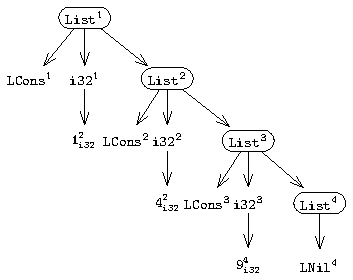
\includegraphics[scale=1]{chapters/figures/figParseTreeList3.pdf}}
\end{center}
\vspace{-15px}
\caption{\label{fig:listParseTree}{\tt List = LNil | \newline LCons(i32, List)}}
\end{subfigure}
\begin{subfigure}[b]{1\textwidth}
\begin{center}
{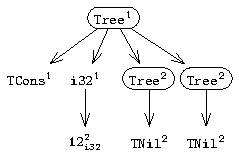
\includegraphics[scale=1.1]{chapters/figures/figParseTreeTree2.pdf}}
\end{center}
\vspace{-15px}
\caption{\label{fig:treeParseTree}{\tt Tree = TNil | \newline TCons(i32, Tree, Tree)}}
\end{subfigure}%
\end{minipage}%
\begin{minipage}[c]{0.55\textwidth}
\begin{subfigure}[b]{1\textwidth}
\begin{center}
{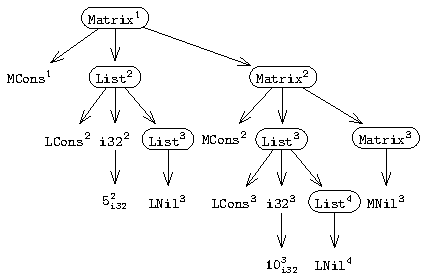
\includegraphics[scale=1]{chapters/figures/figParseTreeMatrix2.pdf}}
{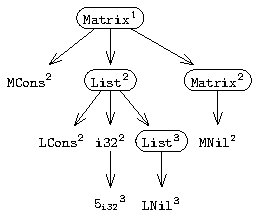
\includegraphics[scale=1.1]{chapters/figures/figParseTreeMatrix1.pdf}}
\end{center}
\vspace{-15px}
\caption{\label{fig:matrixParseTree}{\tt Matrix = MNil | \newline MCons(List, Matrix)}}
\end{subfigure}%
\end{minipage}%
\caption{\label{fig:parseTrees}Parsed Trees with depths (shown as superscript) for three values, each of ADT type {\tt List}, {\tt Tree}, and {\tt Matrix} respectively.}
\end{figure}
